\documentclass[twoside,10pt]{article}
\usepackage{/Users/bradenhoagland/latex/styles/toggles}
%\toggletrue{sectionbreaks}
%\toggletrue{sectionheaders}
\newcommand{\docTitle}{Math 611 - HW 5}
\usepackage{/Users/bradenhoagland/latex/styles/common}
\importStyles{modern}{rainbow}{boxy}

%\renewcommand{\theenumi}{\alph{enumi}}

\begin{document}
%\tableofcontents

% ------------------------------
% 1.3: 5
% ------------------------------
\begin{exer}[1.3: 5]
	For all covering spaces of the comb-ish space in the text, the left edge lifts homeomorphically. Deduce that there is no simply connected covering space.
\end{exer}

\textbf{Left edge lifts homeomorphically:} Suppose we have a covering space $\tilde{X}\stackrel{p}{\to } X$. Take an open cover of the left edge of the space (call it $L$) by evenly covered neighborhoods. Since $L=I$, which is compact, so we can take a finite subcover. We will now construct a homeomorphic lift of $L$ by gluing together specific parts of the lifts of each open set in this finite subcover.

\begin{figure}[H]
	\centering
	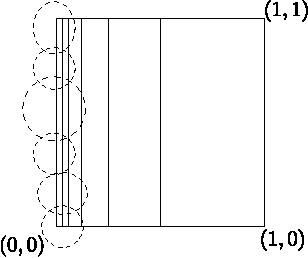
\includegraphics[scale=1]{fig/5a.pdf}
	%\caption{}
\end{figure}

There is necessarily an evenly covered neighborhood of $(0,0)$; call it $U_1$. Its lift is a disjoint union of homeomorphic (via $p$) copies of itself. Choose one of these homeomorphic sets and call it $\tilde{U}_1$. Now choose another evenly covered set in the subcover of $L$ that intersects $U_1$, and call it $U_2$. It too lifts to a disjoint union of homeomorphic sets in $\tilde{X}$, and we must choose one that ``agrees" with $\tilde{U}_1$.

Since we've already chosen $\tilde{U}_1$, we've fixed the basepoint to which $(0,0)$ lifts. Then the path $L \isct U_1$ (starting at $(0,0)$) lifts uniquely to $\tilde{X}$ with endpoint $x \in \tilde{U}_1$. We can then choose one of the disjoint homeomorphic lifts of $U_2$ (call it $\tilde{U}_2)$ such that $x \in \tilde{U}_1 \isct \tilde{U}_2$ and $p(x) = U_1 \isct U_2$. We repeat this process inductively, eventually lifting all of $L$ since there are a finite number of $U_i$ in our subcover of $L$.

We now claim that $p|_{\tilde{U}_1 \uni \cdots \uni \tilde{U}_n}$ is a homeomorphism $\tilde{U}_1 \uni \cdots \uni \tilde{U}_n \to U_1\uni\cdots\uni U_n$. To show this, it suffices to show that $p|_{\tilde{U}_1 \uni \tilde{U}_2}$ is a homeomorphism $\tilde{U}_1 \uni \tilde{U}_2 \to U_1\uni U_2$: since we have finitely many $\tilde{U}_i$, we can extend this result to $n$ of them through induction.

By construction, $p$ agrees on the intersection of the $\tilde{U}_i$, so we can apply the pasting lemma to get a new continuous map on their union. But to ensure that it is still an isomorphism, we can show that it is still bijective, from which we can create an explicit continuous inverse.

Consider $V := U_1 \isct U_2$, which is evenly covered by $p|_{V}$. By construction, $V \subset p(\tilde{U}_1\isct\tilde{U}_2)$, and we always have $p(\tilde{U}_1 \isct \tilde{U}_2) \subset p(\tilde{U}_1) \isct P(\tilde{U}_2) = U_1 \isct U_2 = V$, so $p(\tilde{U}_1 \isct \tilde{U}_2)=V$. The map
\[
	q(x) = 
	\begin{cases}
		p|_{\tilde{U}_1}^{-1}(x) & \text{ if } x \in U_1,\\
		p|_{\tilde{U}_2}^{-1}(x) & \text{ if } x \in U_2
	\end{cases}
\] is then a well-defined inverse of $p|_{\tilde{U}_1 \uni \tilde{U}_2}$, so it's an isomorphism.

\textbf{No simply connected covering space:} Take a neighborhood $U$ of $L$ that lifts homeomorphically to $\tilde{X}$. It is necessarily the union of open balls in $\mathbb{R}^{2}$ intersected with $X$. Since for all $r \in \mathbb{R}$, we can always find an $n \in \mathbb{N}$ such that $1/n < r$, our neighborhood $U$ will always contain come other vertical line in $X$. This means that there will be a noncontractible loop in $U$. Since $U$ lifts homeomorphically, there is a noncontractible loop in $\tilde{X}$, so $\pi_1(\tilde{X}) \neq 1$.

\newpage

% ------------------------------
% 1.3: 8
% ------------------------------
\begin{exer}[1.3: 8]
$\tilde{X},\tilde{Y}$ are simply connected covering spaces of $X$ and $Y$, which are path connected and locally path connected. Show that $X \simeq Y \implies \tilde{X} \simeq \tilde{Y}$.
\end{exer}

The general strategy of this proof will be to appy the lifting criterion to maps $\tilde{X}\to \tilde{Y}$ and $\tilde{Y}\to \tilde{X}$, then show that their compositions are homotopic to the relevant identity map. Suppose the homotopy $X \simeq Y$ is given by the following maps.
\[
\begin{tikzcd}
	X,x_0 \rar[bend left]{f} & Y,y_0 \lar[bend left]{g}
\end{tikzcd}
\] 

First we show that $\tilde{X}$ and $\tilde{Y}$ are locally path connected. We do this only for $\tilde{X}$, as the proof for $\tilde{Y}$ is identical. Fix a point $\tilde{x} \in \tilde{X}$ and take any neighorhood $\tilde{U}$ of it, then $p(\tilde{U})$ is neighborhood of $p(\tilde{x})$ since covering maps are open maps. Then since $X$ is locally path connected, there's some path connected neighborhood $V \subset p(\tilde{U})$ of $p(\tilde{x})$. But since $X$ is covered by evenly covered maps, there is some evenly covered $W$ such that $p(\tilde{x}) \in W \subset V$. Thus $p^{-1}(W) \subset U$ is a path connected neighborhood of $\tilde{x}$, so $\tilde{X}$ is locally path connected.

Denote the covering maps of $\tilde{X}$ and $\tilde{Y}$ by $p_X$ and $p_Y$, respectively. Since $\tilde{X}$ and $\tilde{Y}$ are both assumed to be simply connected, they are certainly both path connected. And since their fundamental groups are trivial, $(f\circ p_X)_{*}(\pi_1(X,x_0)) = (g\circ p_Y)_{*}(\pi_1(Y,y_0))=1$. This means that we can apply the lifting criterion, giving the diagram below.

\[
\begin{tikzcd}
	\tilde{X},\tilde{x}_0 \rar[dashed]{\tilde{f}} \dar{p_X} & \tilde{Y}, \tilde{y}_0 \rar[dashed]{\tilde{g}} \dar{p_Y} & \tilde{X}, (\tilde{g}\tilde{f})(\tilde{x}_0) \dar{p_X} \\
	X,x_0 \rar{f} & Y, y_0 \rar{g} & X, (gf)(x_0)
\end{tikzcd}
\] 
By assumption, there is some homotopy $F:X\times I\to X$ between $\id_{X}$ and $gf$. We now want to show that it lifts to a homotopy $\tilde{F}$ between $\id_{\tilde{X}}$ and $\tilde{g} \tilde{f}$. Consider the following diagram.
\[
\begin{tikzcd}
	\tilde{X}\times I \rar{p_X \times \id_{X}} & X \times I \rar{F} & X
\end{tikzcd}
\] For $\left\{ 0 \right\} \subset I$, we have $F\circ (p_X \times \id_{I}) = F_0\circ p_X = p_X$ since $F_0 = \id_{X}$. Thus the identity certainly lifts $F \circ (p_X \times \id_{I})$ to $\tilde{X}$ on $\left\{ 0 \right\}\subset I$. Then by the homotopy lifting property, this extends to a homotopy $\tilde{F}:\tilde{X}\times I \to \tilde{X}$. We just showed that $\tilde{F}_0 = \id_{\tilde{X}}$, but we still have to show that $\tilde{F}_1 = \tilde{g} \tilde{f}$. Consider the path in $\tilde{X}$ given by $\tilde{F}(\tilde{x}_0, \cdot)$ for some fixed $\tilde{x}_0$.

\begin{figure}[H]
	\centering
	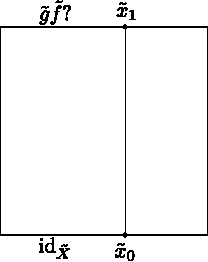
\includegraphics[scale=1]{fig/8.pdf}
	%\caption{}
\end{figure}

This path must be a lift of a path from $x_0$ to $(gf)(x_1)$ in $X$, which lifts (uniquely!) to $\tilde{X}$ (see the figure below). Since a path ending at $\tilde{g}\tilde{f}(\tilde{x}_0)$ is certainly such a lift, uniqueness means that this must be the lift. Thus $\tilde{F}_1 = \tilde{g} \tilde{f}$.

\begin{figure}[H]
	\centering
	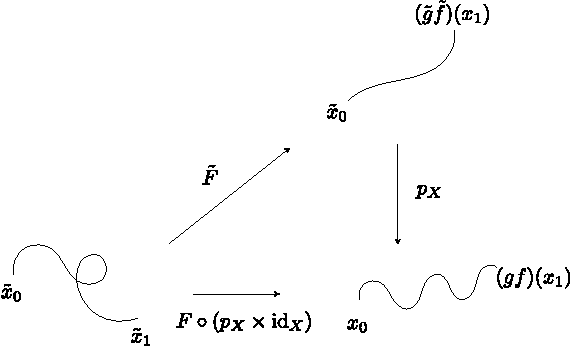
\includegraphics[scale=1]{fig/8b.pdf}
	%\caption{}
\end{figure}

Thus $\tilde{F}$ is the homotopy showing $\tilde{X} \simeq \tilde{Y}$.

\newpage

% ------------------------------
% 1.3: 10
% ------------------------------
\begin{exer}[1.3: 10]
Find all 2/3 sheeted connected covering spaces of $S^{1}\vee S^{1}$ up to isomorphism without basepoints.
\end{exer}

$S^{1}\vee S^{1}$ has a basepoint $x$ where both circles coincide. If a covering space of $S^{1}\vee S^{1}$ has $n$ sheets, then it must have exactly $n$ points that map to $x$ under the covering map. We can then proceed to find all the $n$-sheeted covering spaces more or less combinatorially. Below, we assume that $S^{1}\vee S^{1}$ is given by the following.
\begin{figure}[H]
	\centering
	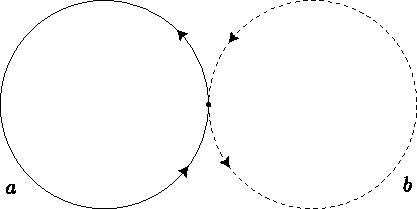
\includegraphics[scale=1]{fig/10.pdf}
	%\caption{}
\end{figure}
I'll abuse notation below by using $a$ and $b$ to refer to disjoint copies of their preimages in the various covering spaces.

\textbf{2 sheets:}
We start with 2 empty vertices $x_1$ and $x_2$ and wish to connect them to create a 2-oriented graph. Suppose $a$ goes from $x_1$ to $x_2$, then there must be another $a$ going from $x_2$ to $x_1$ since both vertices must have a neighborhood with $a$ both coming in and going out. There are then two options for how to treat $b$. Either both copies of $b$ stay at their own vertex or both go between vertices. Both options are shown below.
\begin{figure}[H]
	\centering
	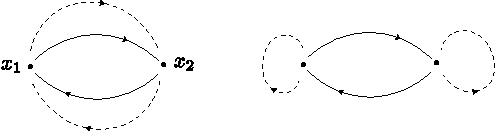
\includegraphics[scale=1.3]{fig/10b.pdf}
	%\caption{}
\end{figure}
Now suppose $a$ does not run between vertices but rather has two disjoint copies, one at each vertex. Then in order to remain connected, $b$ must run between the vertices. We then get the below covering space.
\begin{figure}[H]
	\centering
	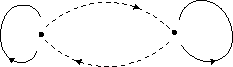
\includegraphics[scale=1.3]{fig/10c.pdf}
	%\caption{}
\end{figure}
If we repeat all the above logic with the roles of $a$ and $b$ reversed, we get the same three spaces. Thus these are then all the 2-sheeted connected covering spaces of $S^{1}\vee S^{1}$.

\textbf{3 sheets:} I don't have digital versions of these covering spaces, as my patience with the software I was using was wearing thin. Instead, see attached figure A. The general concept here is the same as in the previous part, except there are three vertices instead of two and thus more valid choices at each step.

\begin{enumerate}
	\item[i.] Suppose $a$ goes between $x_1$ and $x_2$, then to stay connected, we need $b$ to run between $x_2$ and $x_3$. This then forces $a$ to loop at $x_3$ and $b$ to loop at $x_1$.

	\item[ii.] Instead of going back and forth between $x_1$ and $x_2$, suppose $a$ goes from $x_1$ to $x_2$ and then $x_2$ to $x_3$. This forces $a$ to return to $x_1$ from $x_3$. We can do the same with $b$.

	\item[iii.] Instead of doing the same with $b$, we reverse the orientation of each $b$.

	\item[iv.] There was no reason we had to mirror $a$ with $b$ in (ii) and (iii). We could have instead had $b$ run between $x_2$ and $x_3$, then loop at $x_1$ (if $b$ runs between $x_1$ and $x_2$ and loops at $x_3$, etc., we're in an isomorphic situation).

	\item[v.] We can reverse the orientation of $a$ in (iv) while fixing $b$.

	\item[vi.] The only possibilies we've yet to exhaust are when $a$ is a loop at $x_1$. In this case, we've seen in (iv) and (v) that we can have $a$ run between the other two vertices. We could've also had it loop at both, though. If we do so with $a$, this forces $b$ to run from $x_1$ to $x_2$, then from $x_2$ to $x_3$, and from $x_3$ to $x_1$.

	\item[vii.] We can swap the orientation of $b$ in (vi).
\end{enumerate}

Of course, we could've done the above with the roles of $a$ and $b$ flipped, but that would give us isomorphic versions of what we've already done.

\newpage

% ------------------------------
% 1.3: 14
% ------------------------------
\begin{exer}[1.3: 14]
Find all connected covering spaces of $\mathbb{R}P^2 \vee \mathbb{R}P^2$.
\end{exer}

We know $\pi_1(\mathbb{R}P^2) = \pi_1(N_1) \cong \ang{a \;|\; \alpha_2}\cong \mathbb{Z}_2$. Since there's a bijection between the conjugacy clases of $\mathbb{Z}_2$ (which are just $1$ and $\mathbb{Z}_2$ itself) and the isomorphism classes of connected covering spaces of $\mathbb{R}P^2$ without basepoint, we know that there are two unique connected covering spaces: $\mathbb{R}P^2$ itself and its universal cover $S^2$. All other covering spaces of $\mathbb{R}P^2$ are then disjoint copies of these two.

Any covering space of $\mathbb{R}P^2 \vee \mathbb{R}P^2$ must restrict to covers of $\mathbb{R}P^2$, so we're limited to building its covering spaces using copies of $\mathbb{R}P^2$ and $S^2$. Suppose we give the two halves of $\mathbb{R}P^2 \vee \mathbb{R}P^2$ the names $a$ and $b$ (attached figure 1). If $x$ is the basepoint of $\mathbb{R}P^2 \vee \mathbb{R}P^2$, then any neighborhood $U$ of $x$ intersects both $A$ and $B$, so this must also be true for any $\tilde{x} \in \tilde{p}^{-1}(x)$, where $p:\tilde{X}\to X$ is a covering map.

There are several possibilities for how to combine $\mathbb{R}P^2$ and $S^2$, as shown in attached figure 2. We can then enumerate all possible connected covering spaces of $\mathbb{R}P^2 \vee \mathbb{R}P^2$, which are drawn in attached figure 3 in the order I discuss them below.

We start with $\mathbb{R}P^2 \vee \mathbb{R}P^2$ itself. We then have every possible connected way of combining $S^2$ and $\mathbb{R}P^2$. Any copy of $\mathbb{R}P^2$ can only attach to a preimage of $x$ at one point, while $S^2$ must attach at exactly 2 points. Thus we can form chains of spheres, with $\mathbb{R}P^2$ forming the end of the chain. Note that if the number of spheres in a finite chain is odd, alternating how we label them gives two different covering spaces.

We don't have to include $\mathbb{R}P^2$ at all, though, giving us finite rings of $2n$ spheres and an infinite chain of spheres (which is the universal cover since it's simply connected).

\newpage

\end{document}
